%Auswertung des Emissionsspektrums
\subsection{Auswertung}
Es soll das R�ntgenspektrum der Kupferanode bei drei unterschiedlichen Beschleunigungsspannungen und mit einem Ni-Filter, bei m�glichst hoher R�ntgenspannung untersucht werden.
Zum beugen der R�ntgenstrahlen wird ein Si(111)-Einkristall verwendet, der Netzebenabstand liegt bei \SI{3,1356}{\angstrom}, entnommen von \cite{si_a}.
Gescannt wird ein Winkelbereich von 15$^\circ$ bis 130$^\circ$, dabei wurden f�r die Beschleunigungsspannung Werte von
\begin{itemize}
\item U = 30kV und A = 10mA
\item U = 40kV und A = 10mA
\item U = 40kV und A = 30mA
\end{itemize}
 verwendet. Dabei ergeben sich die folgenden Plots.
 
 % Plots der Messunge f\"ur die Kupferanode mit unterschiedlichen Beschleunigungsspannungen
In Abb. \ref{fig:spektrum_1} ist das Diffraktogramm f�r U = 30kV und A = 10mA.
 
\begin{figure}[H]
	\centering
  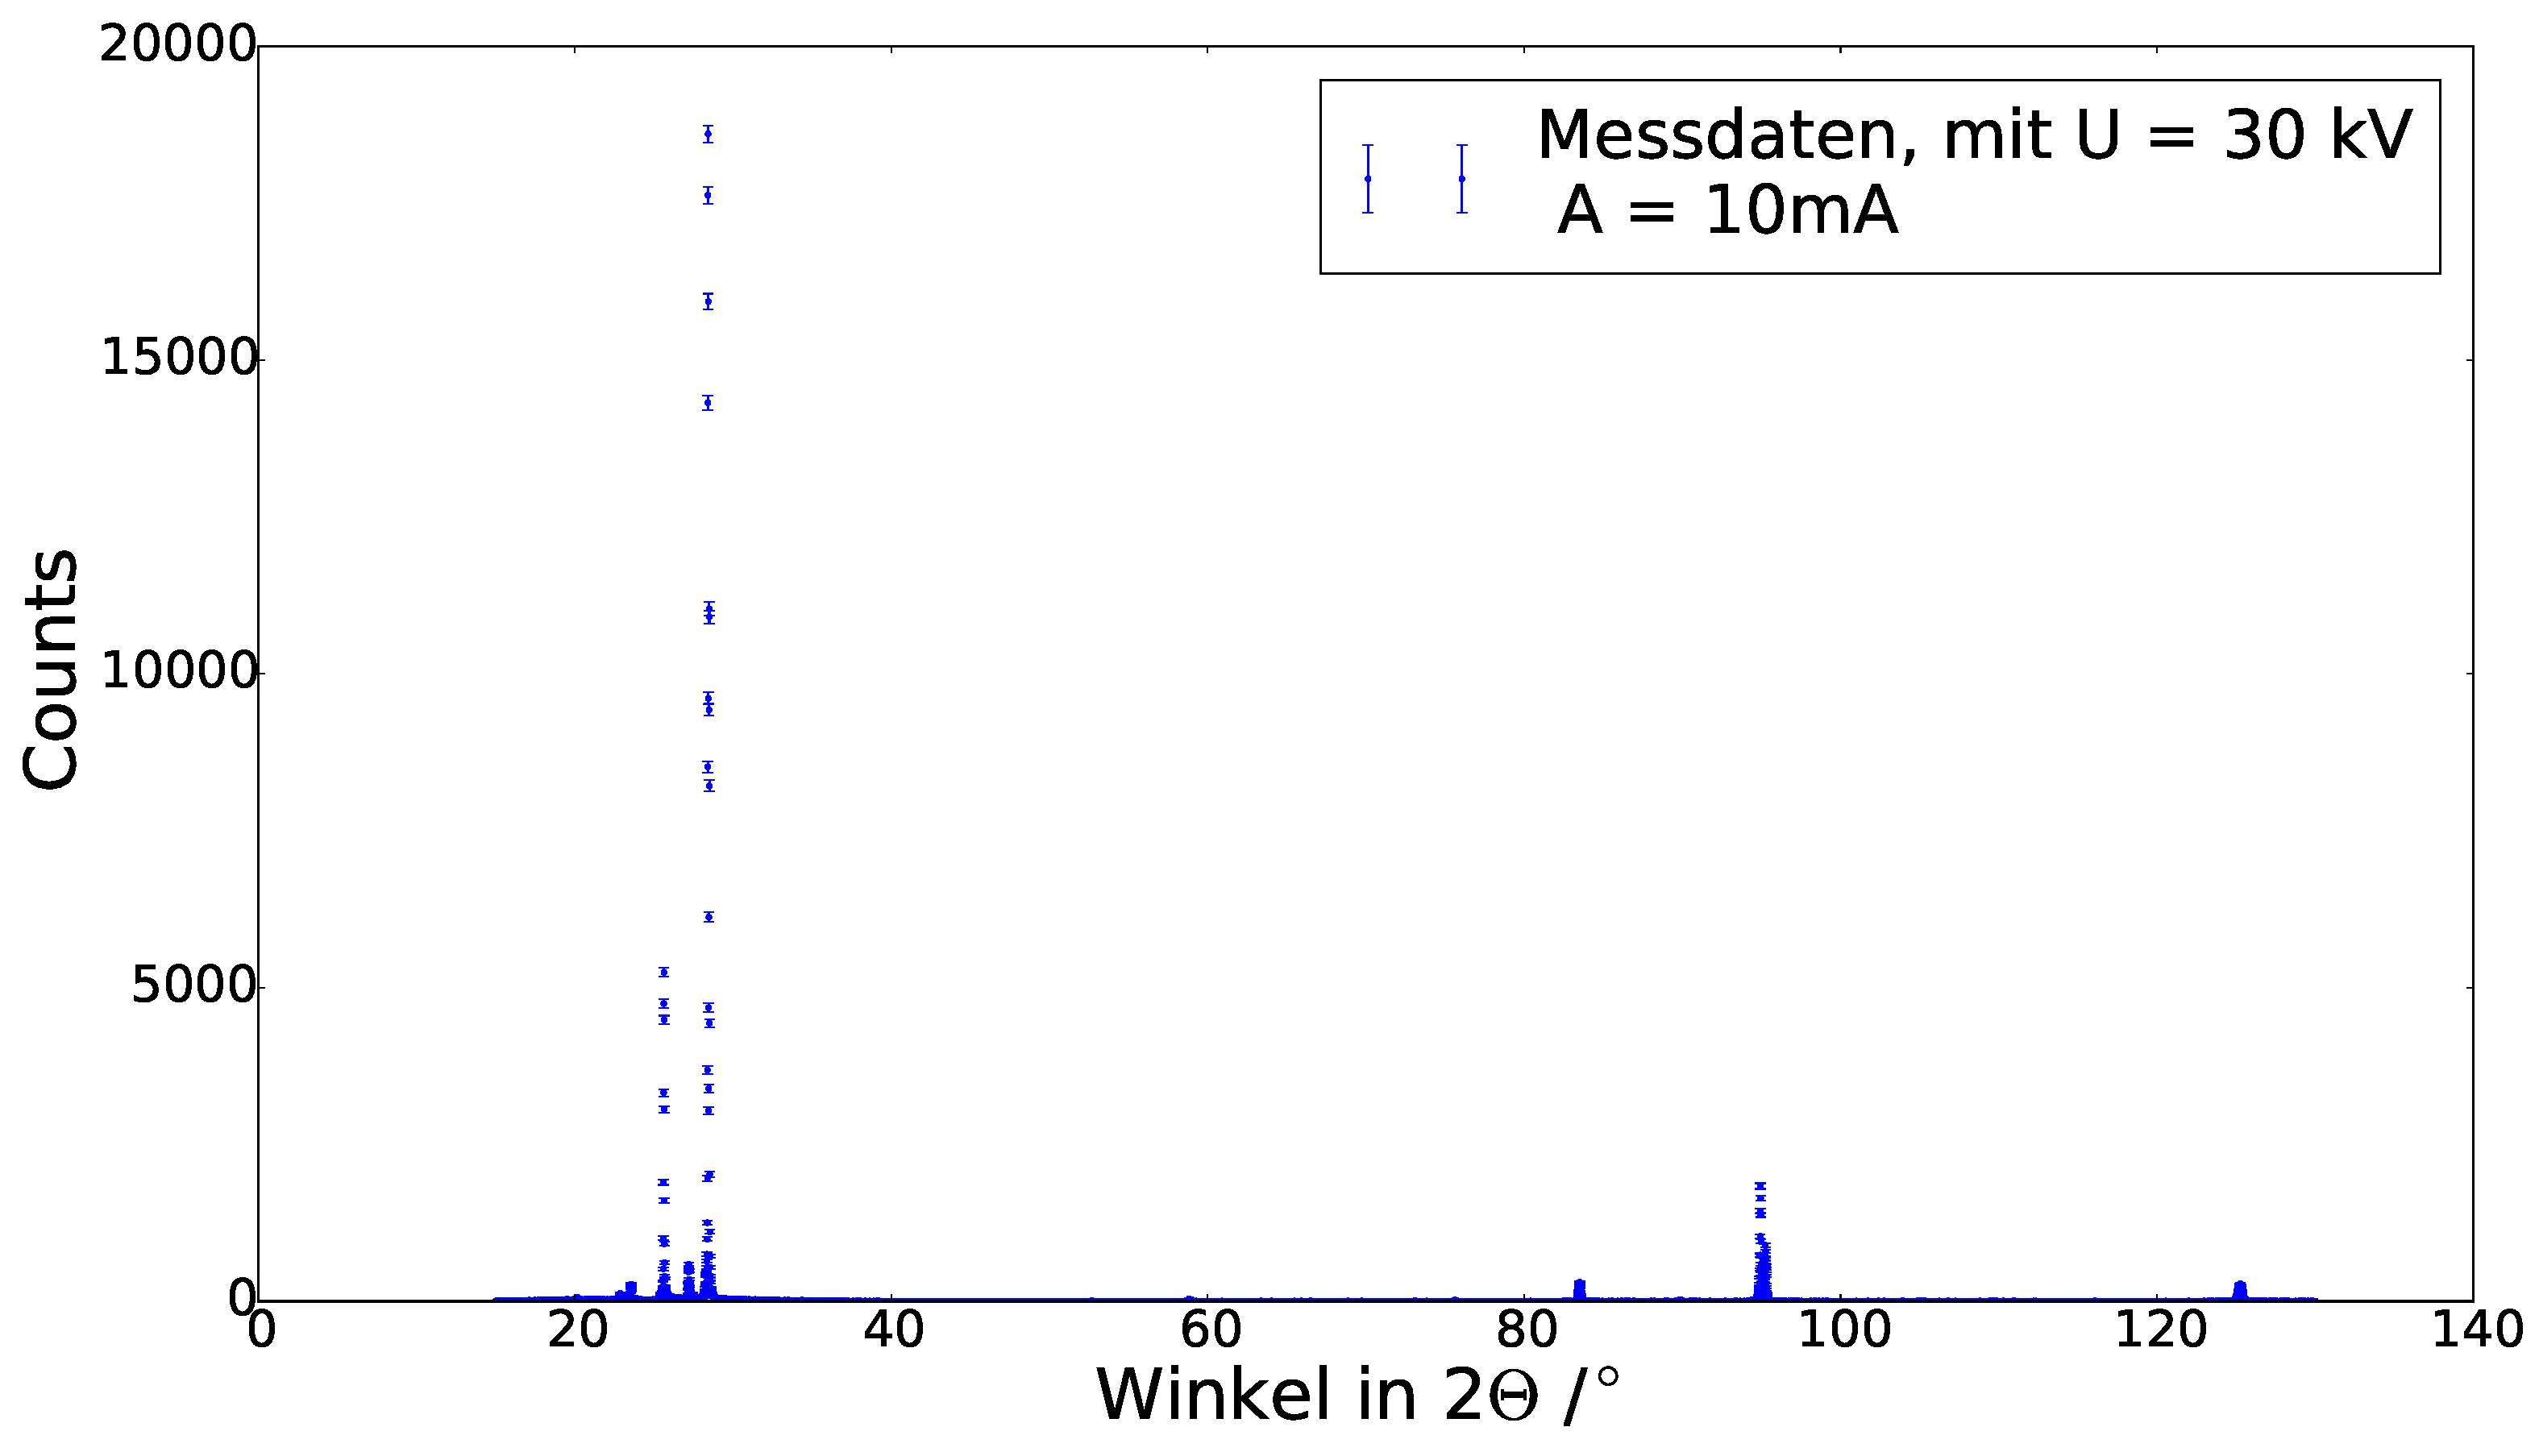
\includegraphics[scale=0.30]{spektrum_1.pdf}
	\caption{Diffraktogramm bei 30kV Beschleunigungsspannung und einem Anodenstrom von 10mA}
	\label{fig:spektrum_1}
\end{figure}

In Abb. \ref{fig:spektrum_2} ist das Diffraktogramm f�r U = 40kV und A = 10mA.
 
\begin{figure}[H]
	\centering
  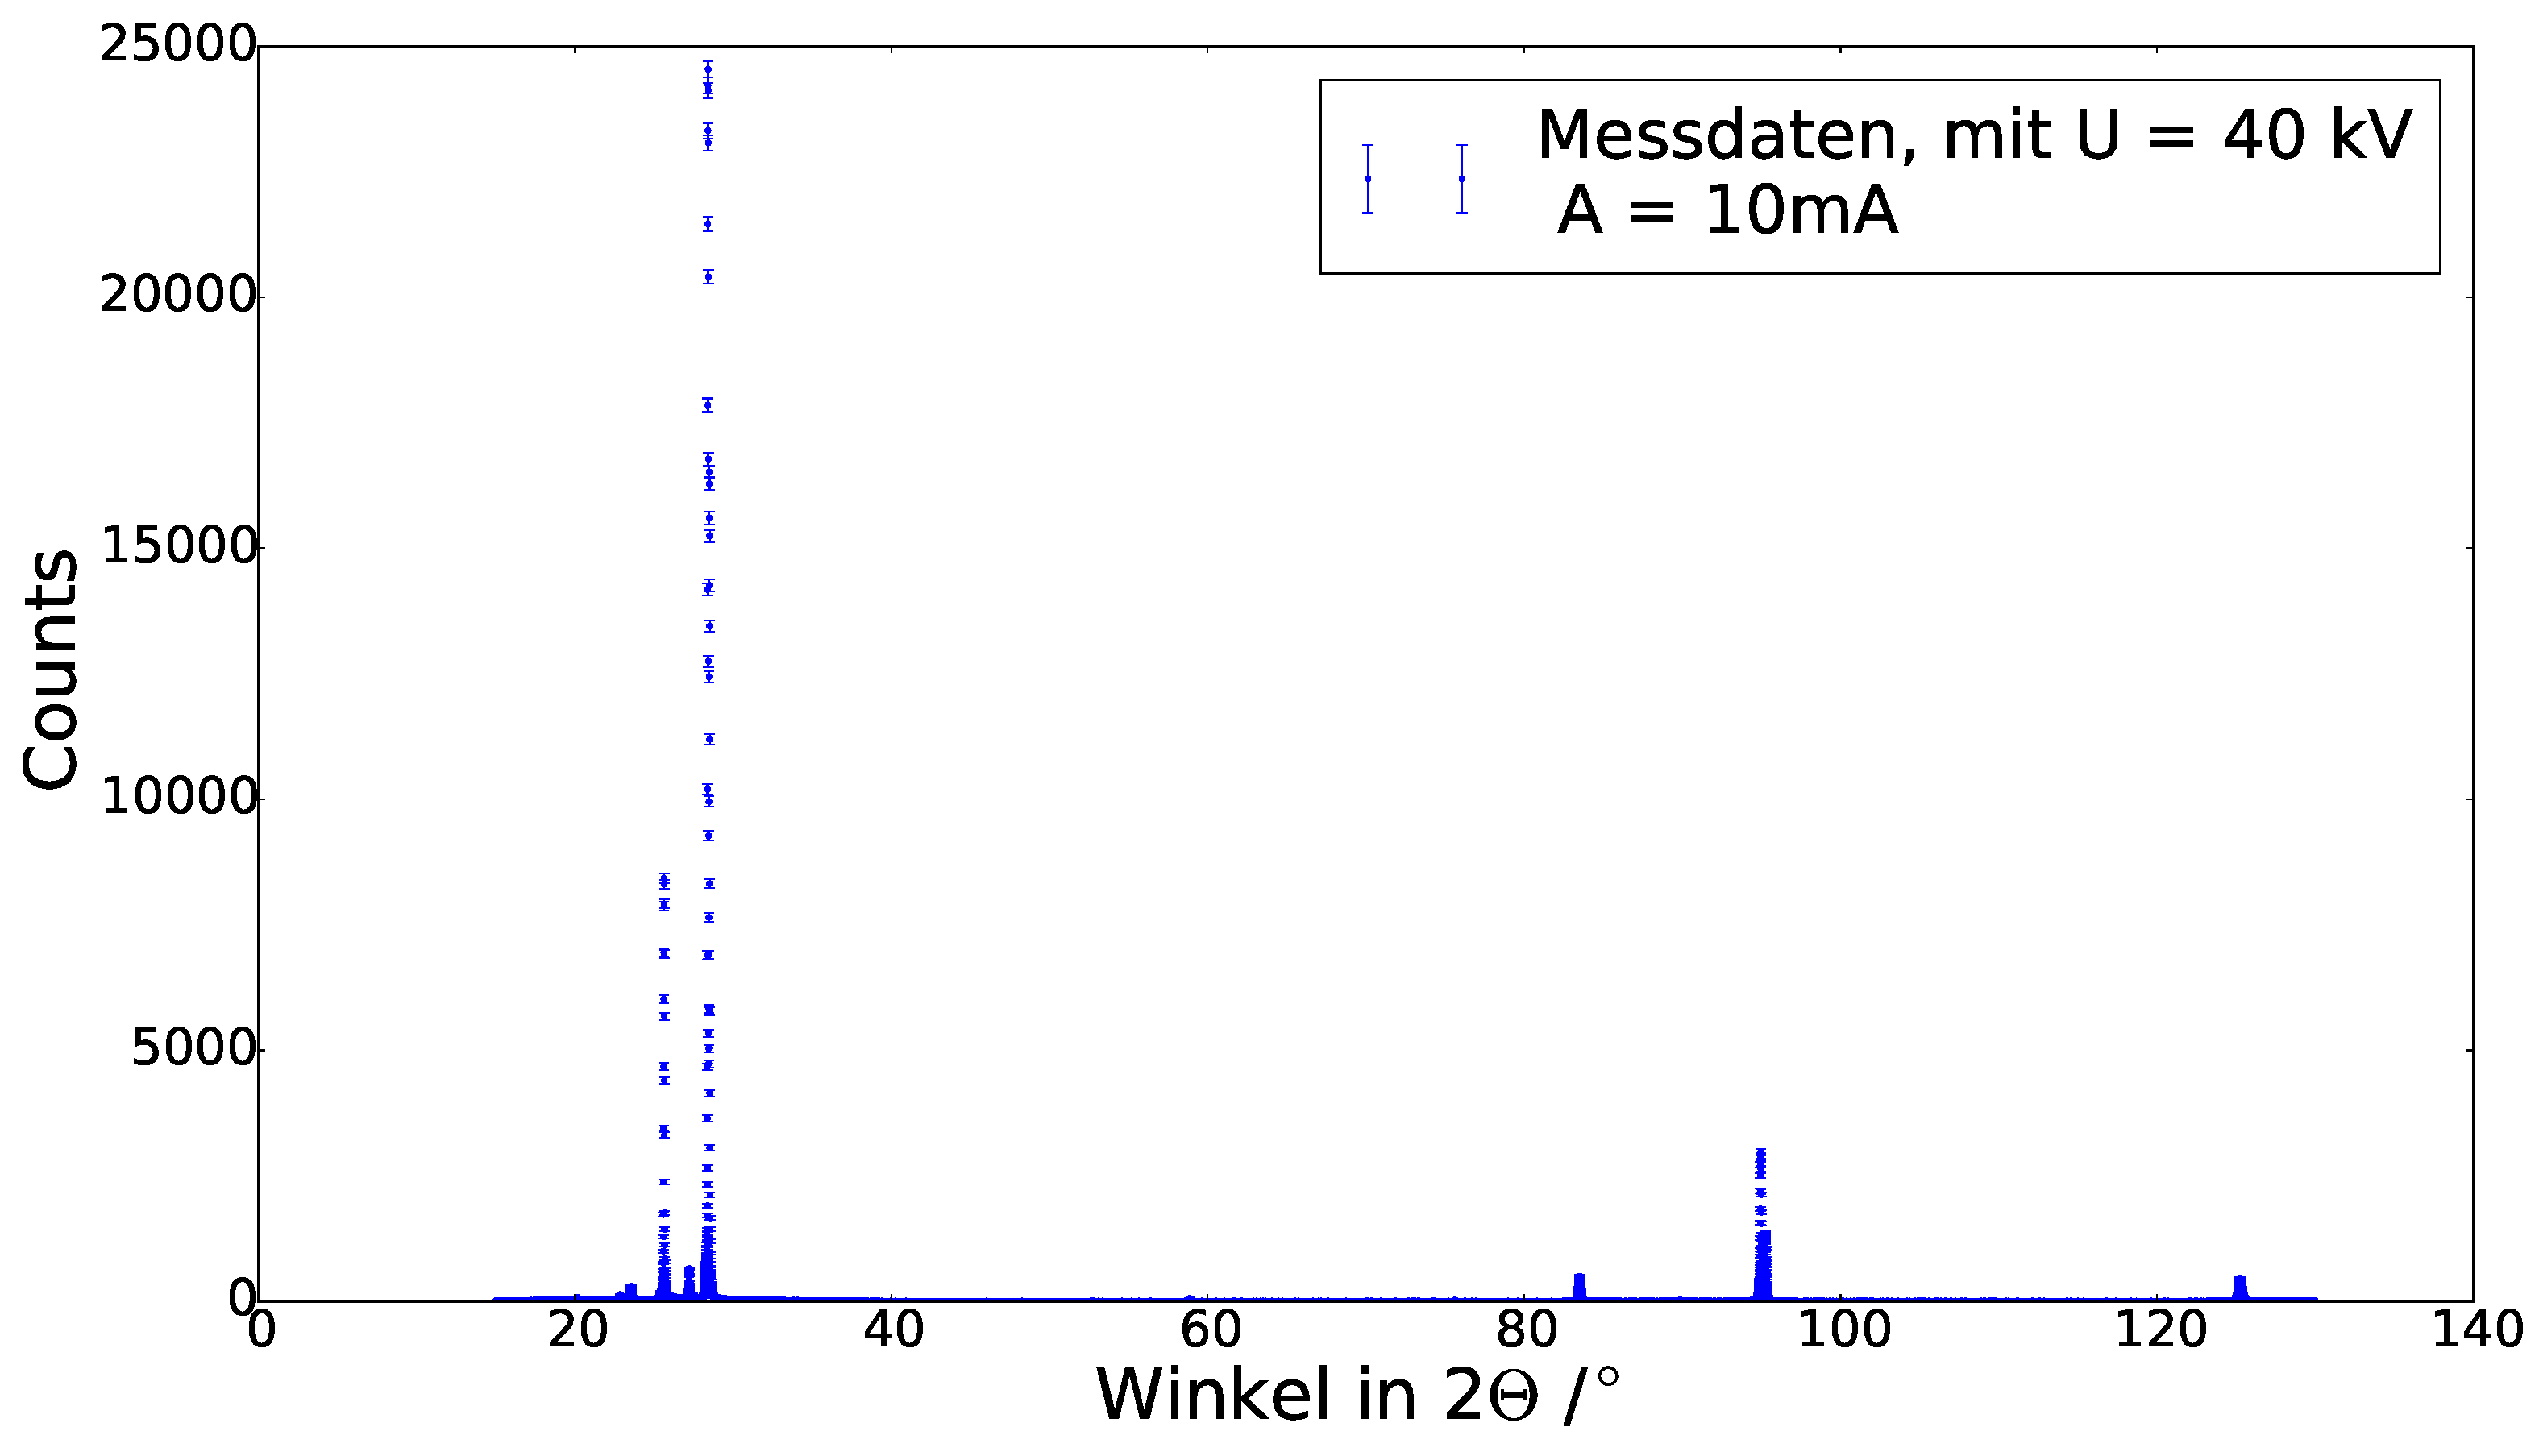
\includegraphics[scale=0.30]{spektrum_2.pdf}
	\caption{Diffraktogramm bei 40kV Beschleunigungsspannung und einem Anodenstrom von 10mA}
	\label{fig:spektrum_2}
\end{figure}

In Abb. \ref{fig:spektrum_3} ist das Diffraktogramm f�r U = 40kV und A = 30mA.

\begin{figure}[H]
	\centering
  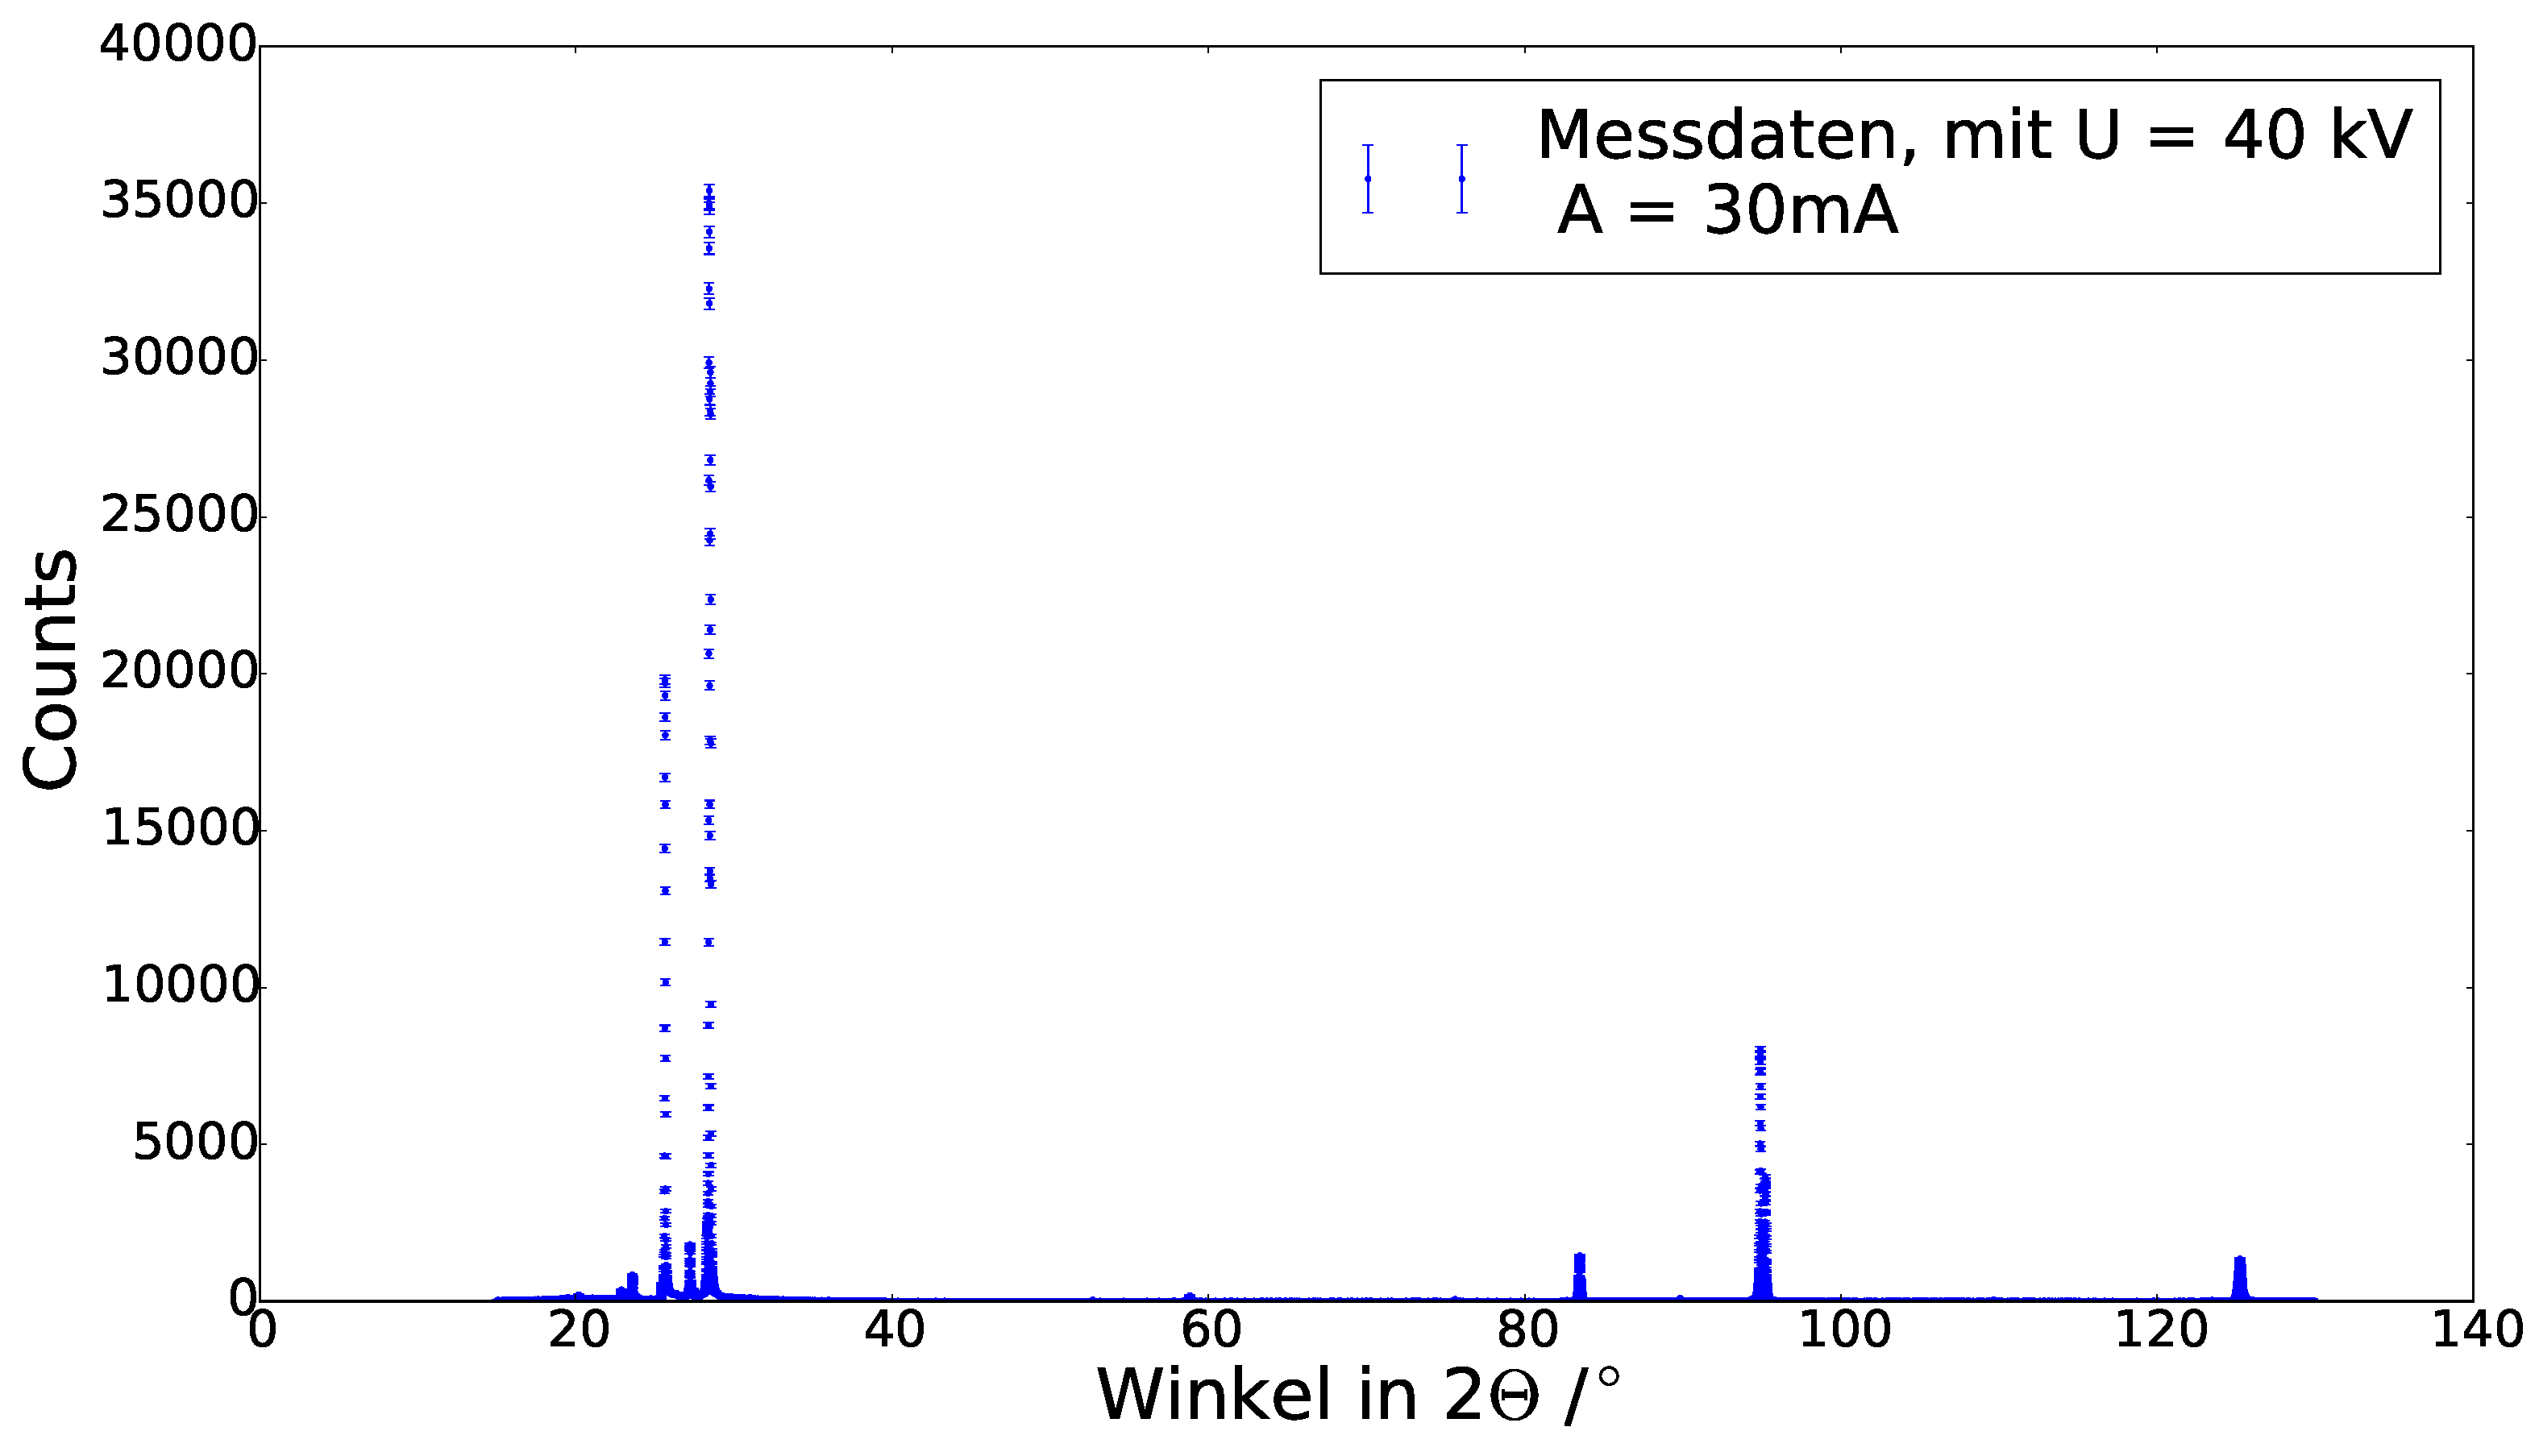
\includegraphics[scale=0.30]{spektrum_3.pdf}
	\caption{Diffraktogramm bei 40kV Beschleunigungsspannung und einem Anodenstrom von 30mA}
	\label{fig:spektrum_3}
\end{figure}
 

Es ist deutlich zu erkennen, das bei steigender Beschleunigungsspannung und Strom die Anzahl der Counts gr��er werden und so die Peaks deutlich von dem Untergrund zu unterscheiden sind.
Um Informationen �ber den Winkel und die Intensit�t zu erhalten, werden die Peaks mit der Voigtverteilung gefittet.
Die Energie wird nach Gleichung  bestimmt, die Counts ergeben sich mit Gleichung ??. Der Fehler wird mit Gleichung ?? bestimmt.

Es ergeben sich die folgenden Ergebnisse:

\begin{table}[H]
\caption{In der Tabelle sind die Messdaten und die daraus bestimmten Energien f�r die unterschiedlichen Cu-Linien und Ordnungen}
\label{tab:ergebnisse_1}
\centering
\begin{tabular}{|c|c|c|c|c|c|c|c|c|}
\hline Cu-Linie & Ordung & 2$\theta^\circ$ & $\Delta$2$\theta^\circ$ & Counts & $\Delta$Counts & E$_{exp}$[eV] & $\Delta$E$_{exp}$[eV] & E$_{literatur}$ \\ 
\hline K$_\beta$ & 1 &  &  &  &  &  &  &  \\ 
\hline K$_{\alpha_1}$ & 1 &  &  &  &  &  &  &  \\ 
\hline K$_{\alpha_2}$ & 1 &  &  &  &  &  &  &  \\ 
\hline K$_\beta$ & 3 &  &  &  &  &  &  &  \\ 
\hline K$_{\alpha_1}$ & 3 &  &  &  &  &  &  &  \\ 
\hline K$_{\alpha_2}$ & 3 &  &  &  &  &  &  &  \\ 
\hline K$_\beta$ & 4 &  &  &  &  &  &  &  \\ 
\hline 
\end{tabular}
\end{table}

%Auswerten der ergebnisse in der Tabelle

Im folgenden sind noch die Gau�-fits mit den bestimmten Parametern zu sehen.

%Plots mit fits einf�gen und Parameter in die Caption schreiben

\subsubsection{Verh�ltnisse}
Aus den bestimmten Peaks sollen die Verh�ltnisse der Cu-Linien und der Ordnungen unter einander.

\begin{table}[H]
\caption{In der Tabelle sind die Verh�ltnisse der einzelnen Cu-Linie und die der Ordnungen zu einander aufgetragen.}
\label{tab:verhaeltnisse}
\centering
\begin{tabular}{|c|c|c|c|c|}
\hline Cu-Linie & Ordnung & Counts & \% der K$_{\alpha_1}$ & \% der 1. Ordnung \\ 
\hline K$_{\alpha_1}$ & 1 &  &  &  \\ 
\hline K$_{\alpha_2}$ & 1 &  &  &  \\ 
\hline K$_\beta$ & 1 &  &  &  \\ 
\hline K$_{\alpha_1}$ & 3 &  &  &  \\ 
\hline K$_{\alpha_2}$ & 3 &  &  &  \\ 
\hline K$_\beta$ & 3 &  &  &  \\ 
\hline K$_\beta$ & 4 &  &  &  \\ 
\hline 
\end{tabular} 
\end{table}

%auswertung der Verhaeltnisse

\subsubsection{Abschw�chung durch den Ni-Filter}
Es soll die Abschw�chung der K$_\beta$-Linie und das Signal-zu-Rausch Verh�ltniss der K$_{\alpha_{1,2}}$-Linie und deren Energie und Energiebreite bestimmt werden.
Mit Verwendung des Filters ergibt sich das Diffrakogramm in Abbildung ??.

%Diffraktogramme mit Fits einf�gen

Es ergibt sich eine Countrate von ?? mit Ni-Filter und ein Count von ?? ohne Ni-Filter. Daraus ergibt sich ein Verh�ltnis von ??.
Das Signal-zu-Rauschverh�ltnis (SNR) wir in [dB] berechnet:

\begin{align}
SNR = 10 \cdot lg \left( \frac{I_{max}}{I_{rausch}} \right)
\end{align}

\subsubsection{Netzebenabstand Si(331)}
Der Si(111)-Einkristall wird nun gegen einen Si(331)-Einkristall ausgetauscht.
Mit den zuvor bestimmten Energien der Cu-Linien soll nach Gleichung ?? der Netzebenabstand bestimmt werden, der Fehler wird mit Gleichung ?? berechnet.
Die Peaks wurden wie zuvor mit der Gau�verteilung gefittet.

%Plot der Peaks mit Fit 

Aus den Messdaten ergeben sich die Werte in Tabelle ??

\begin{table}[H]
\label{tab:si(331)}
\caption{In der Tabelle sind die Ergebnisse zur Bestimmung des Netzebenabstandes von Si(331)}
\centering
\begin{tabular}{|c|c|c|}
\hline Werte & K$_{\alpha_1}$ & K$_{\alpha_2}$ \\ 
\hline 2$\theta [^\circ]$ &  &  \\ 
\hline $\Delta 2\theta [^\circ]$ &  &  \\ 
\hline E[eV] &  &  \\ 
\hline $\Delta$E[eV] &  &  \\ 
\hline d$[\SI{}{\angstrom}]$ &  &  \\ 
\hline $\Delta$d$[\SI{}{\angstrom}]$ &  &  \\ 
\hline 
\end{tabular} 
\end{table}

%Vergleich mit den Literaturwerten


\subsubsection{Netzebenabstand Ge(111)}
Es soll ein Ge(111)-Einkristall untersucht werden, dabei wird wie zuvor vorgegangen.

Aus den Messdaten ergeben sich die Werte in Tabelle ??

\begin{table}[H]
\label{tab:ge(111)}
\caption{In der Tabelle sind die Ergebnisse zur Bestimmung des Netzebenabstandes von Ge(111)}
\centering
\begin{tabular}{|c|c|c|}
\hline Werte & K$_{\alpha_1}$ & K$_{\alpha_2}$ \\ 
\hline 2$\theta [^\circ]$ &  &  \\ 
\hline $\Delta 2\theta [^\circ]$ &  &  \\ 
\hline E[eV] &  &  \\ 
\hline $\Delta$E[eV] &  &  \\ 
\hline d$[\SI{}{\angstrom}]$ &  &  \\ 
\hline $\Delta$d$[\SI{}{\angstrom}]$ &  &  \\ 
\hline 
\end{tabular} 
\end{table}


%Vergleich mit den Literaturwerten



